\section{Regularization Experiments}

Another hyperparameter that may help improve generalization is
regularization. We introduce a new term in the computation of error, $\lambda C$
that measures the \textbf{complexity} of the model. Here, $\lambda$ is the
hyperparameter we tune (typically a small value) to adjust the
strength of the regularization. Altogether, we have a new measure of error

\begin{equation*}
	J = E + \lambda C
\end{equation*}

Here, $C$ can take various forms. Two well-known forms include $L_1$ and $L_2$
regularization.

$L_1$ regularization seeks to minimize $C = |W|$. Therefore,

\begin{equation*}
	\begin{aligned}
		\frac{\partial J}{\partial w_{ij}} & = \nabla E^{(n)}(w_{ij}) + \lambda
		\frac{\partial C}{\partial w_{ij}}                                      \\
		                                   & = \nabla E^{(n)}(w_{ij}) + \lambda
		\text{sign}  (w_{ij})                                                   \\
	\end{aligned}
\end{equation*}

where the matrix of ones $\mathbf{1} \in \mathbb{R}^{i \times j}$. On the other
hand, $L_2$ regularization seeks to minimize $C = \| W \|^2_2$.

\begin{equation*}
	\begin{aligned}
		\frac{\partial J}{\partial w_{ij}} & = \nabla E^{(n)}(w_{ij}) + \lambda
		\frac{\partial C}{\partial w_{ij}}                                        \\
		                                   & = \nabla E^{(n)}(w_{ij}) + 2 \lambda
		w_{ij}                                                                    \\
	\end{aligned}
\end{equation*}

\subsection{Experiments}
In our previous experiments with momentum and early stopping, we achieved a test
accuracy of $96.62\%$ within 7 epochs. We will run our regularization
experiments with approximately $10\%$ more epochs (8 total epochs). We achieve
the following results

\begin{figure}[!ht]
	\centering
	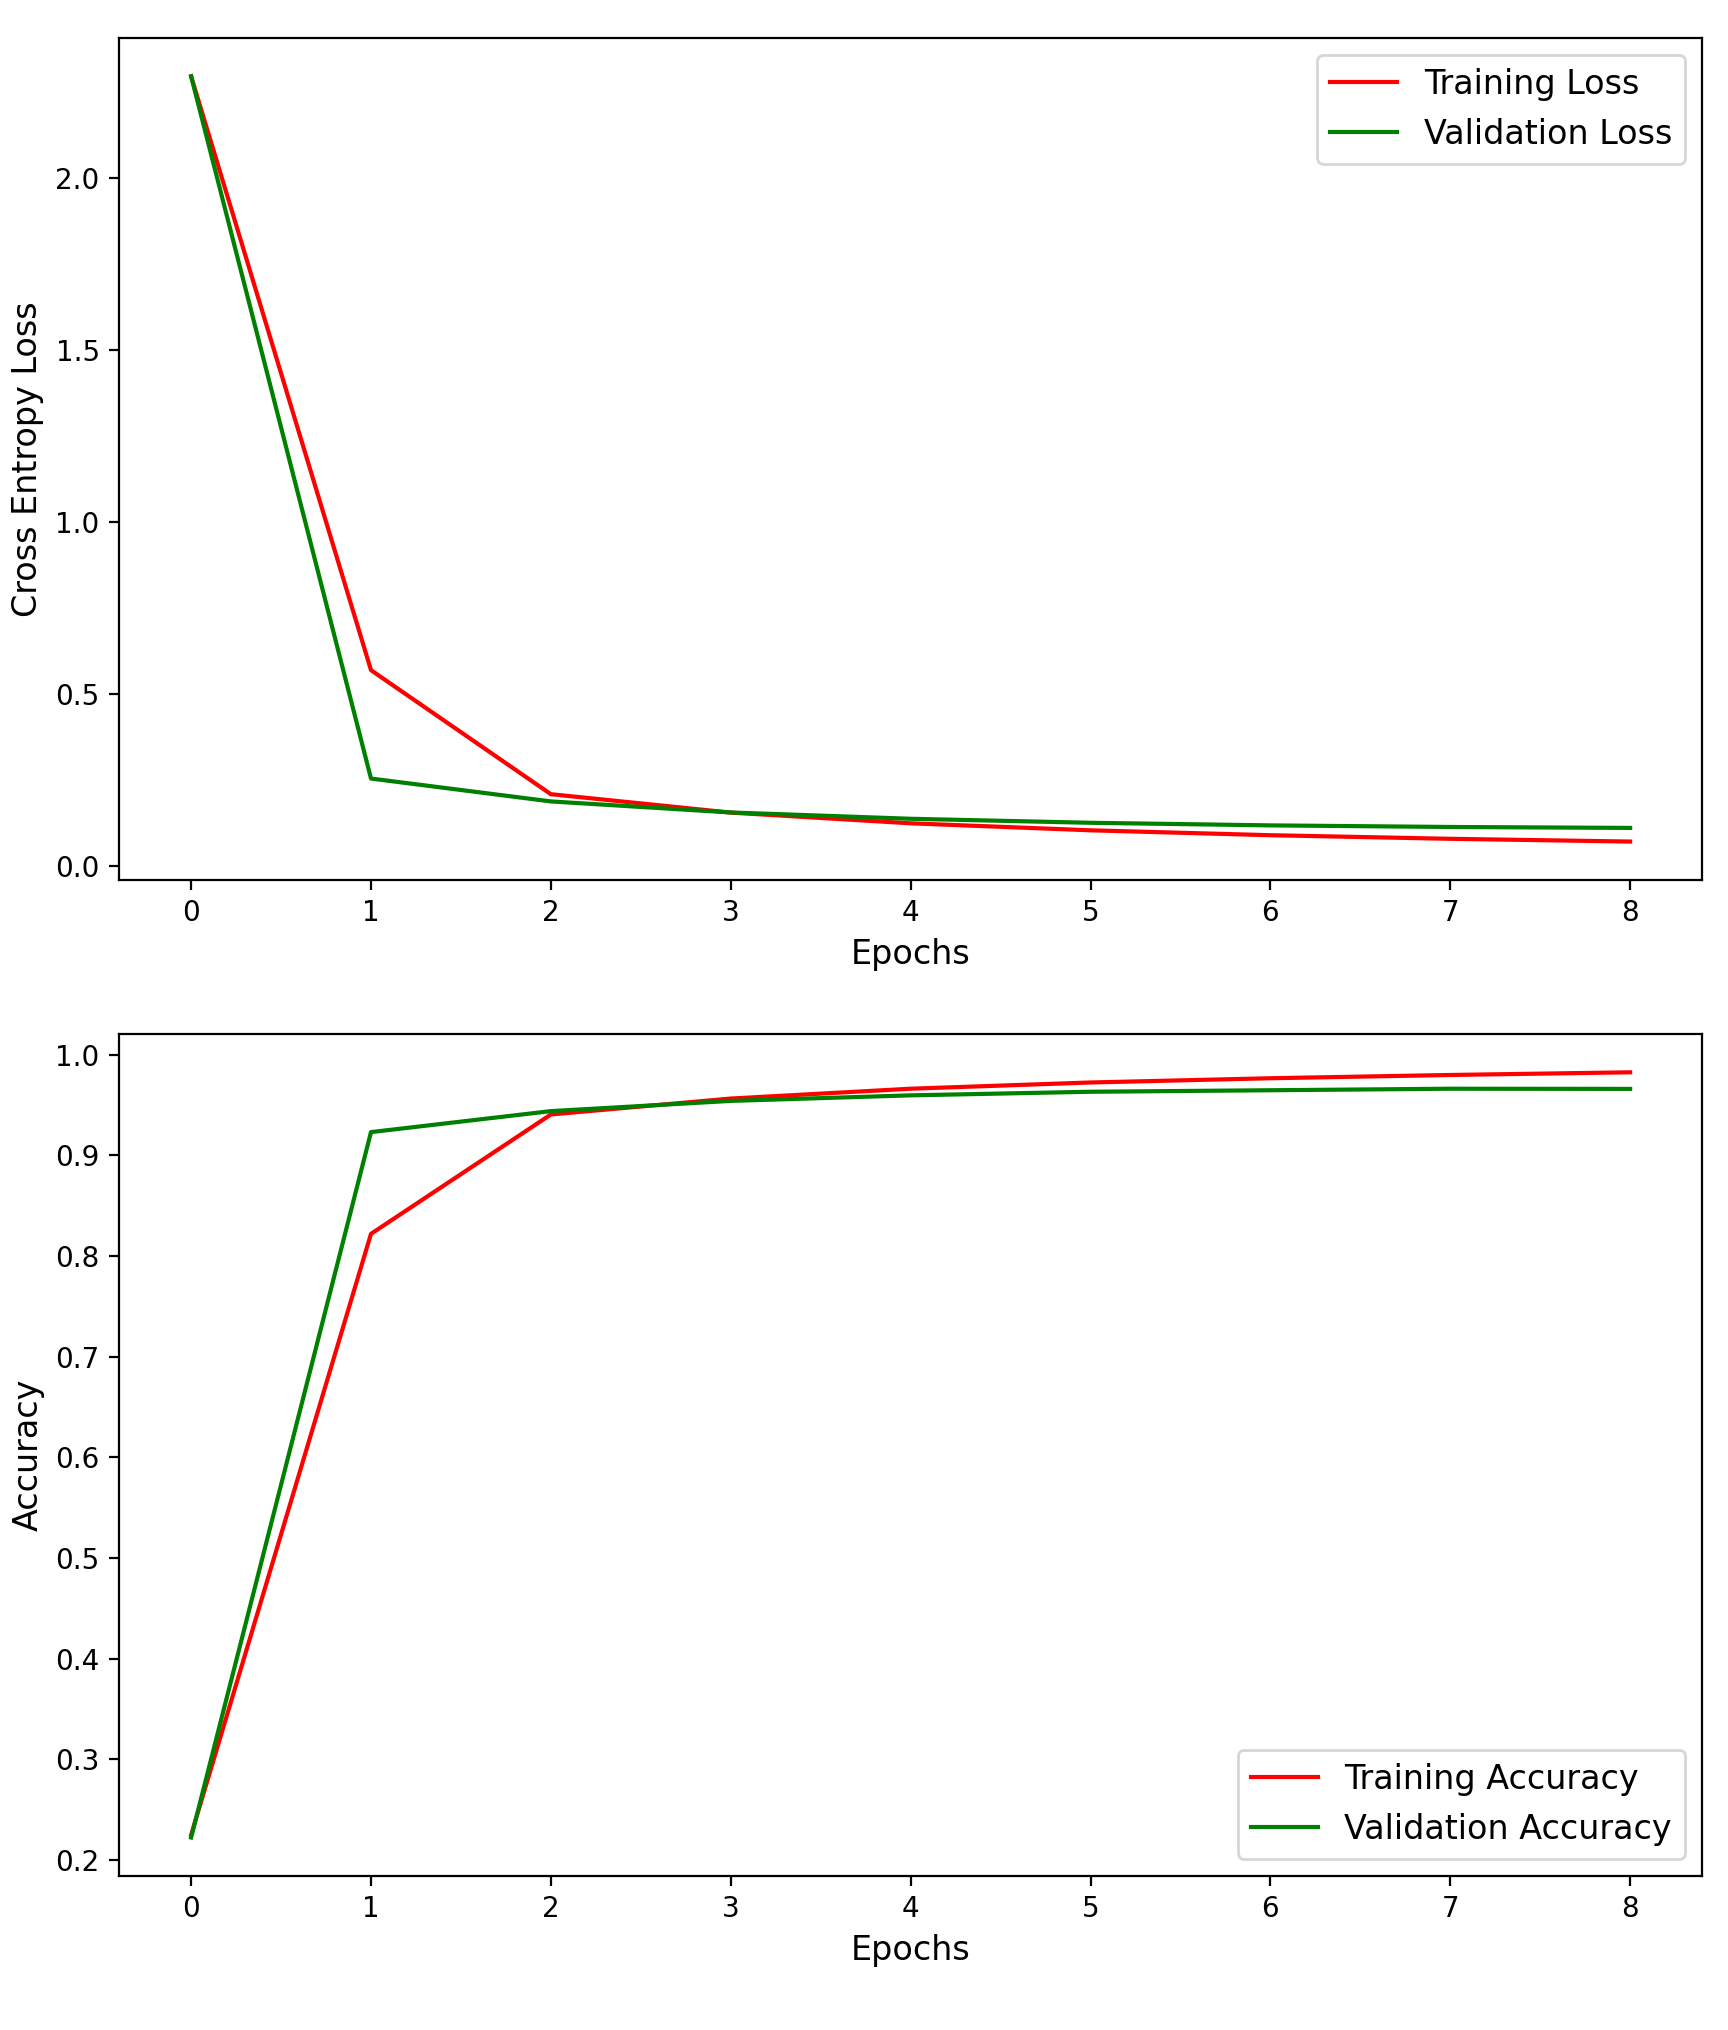
\includegraphics[width=1.0\textwidth]{./images/l1_e2.png}
	\caption{$L_1$ Regularization with $\lambda = 1e^{-2}$}
	\label{fig:l1_1e2}
\end{figure}

\begin{figure}[!ht]
	\centering
	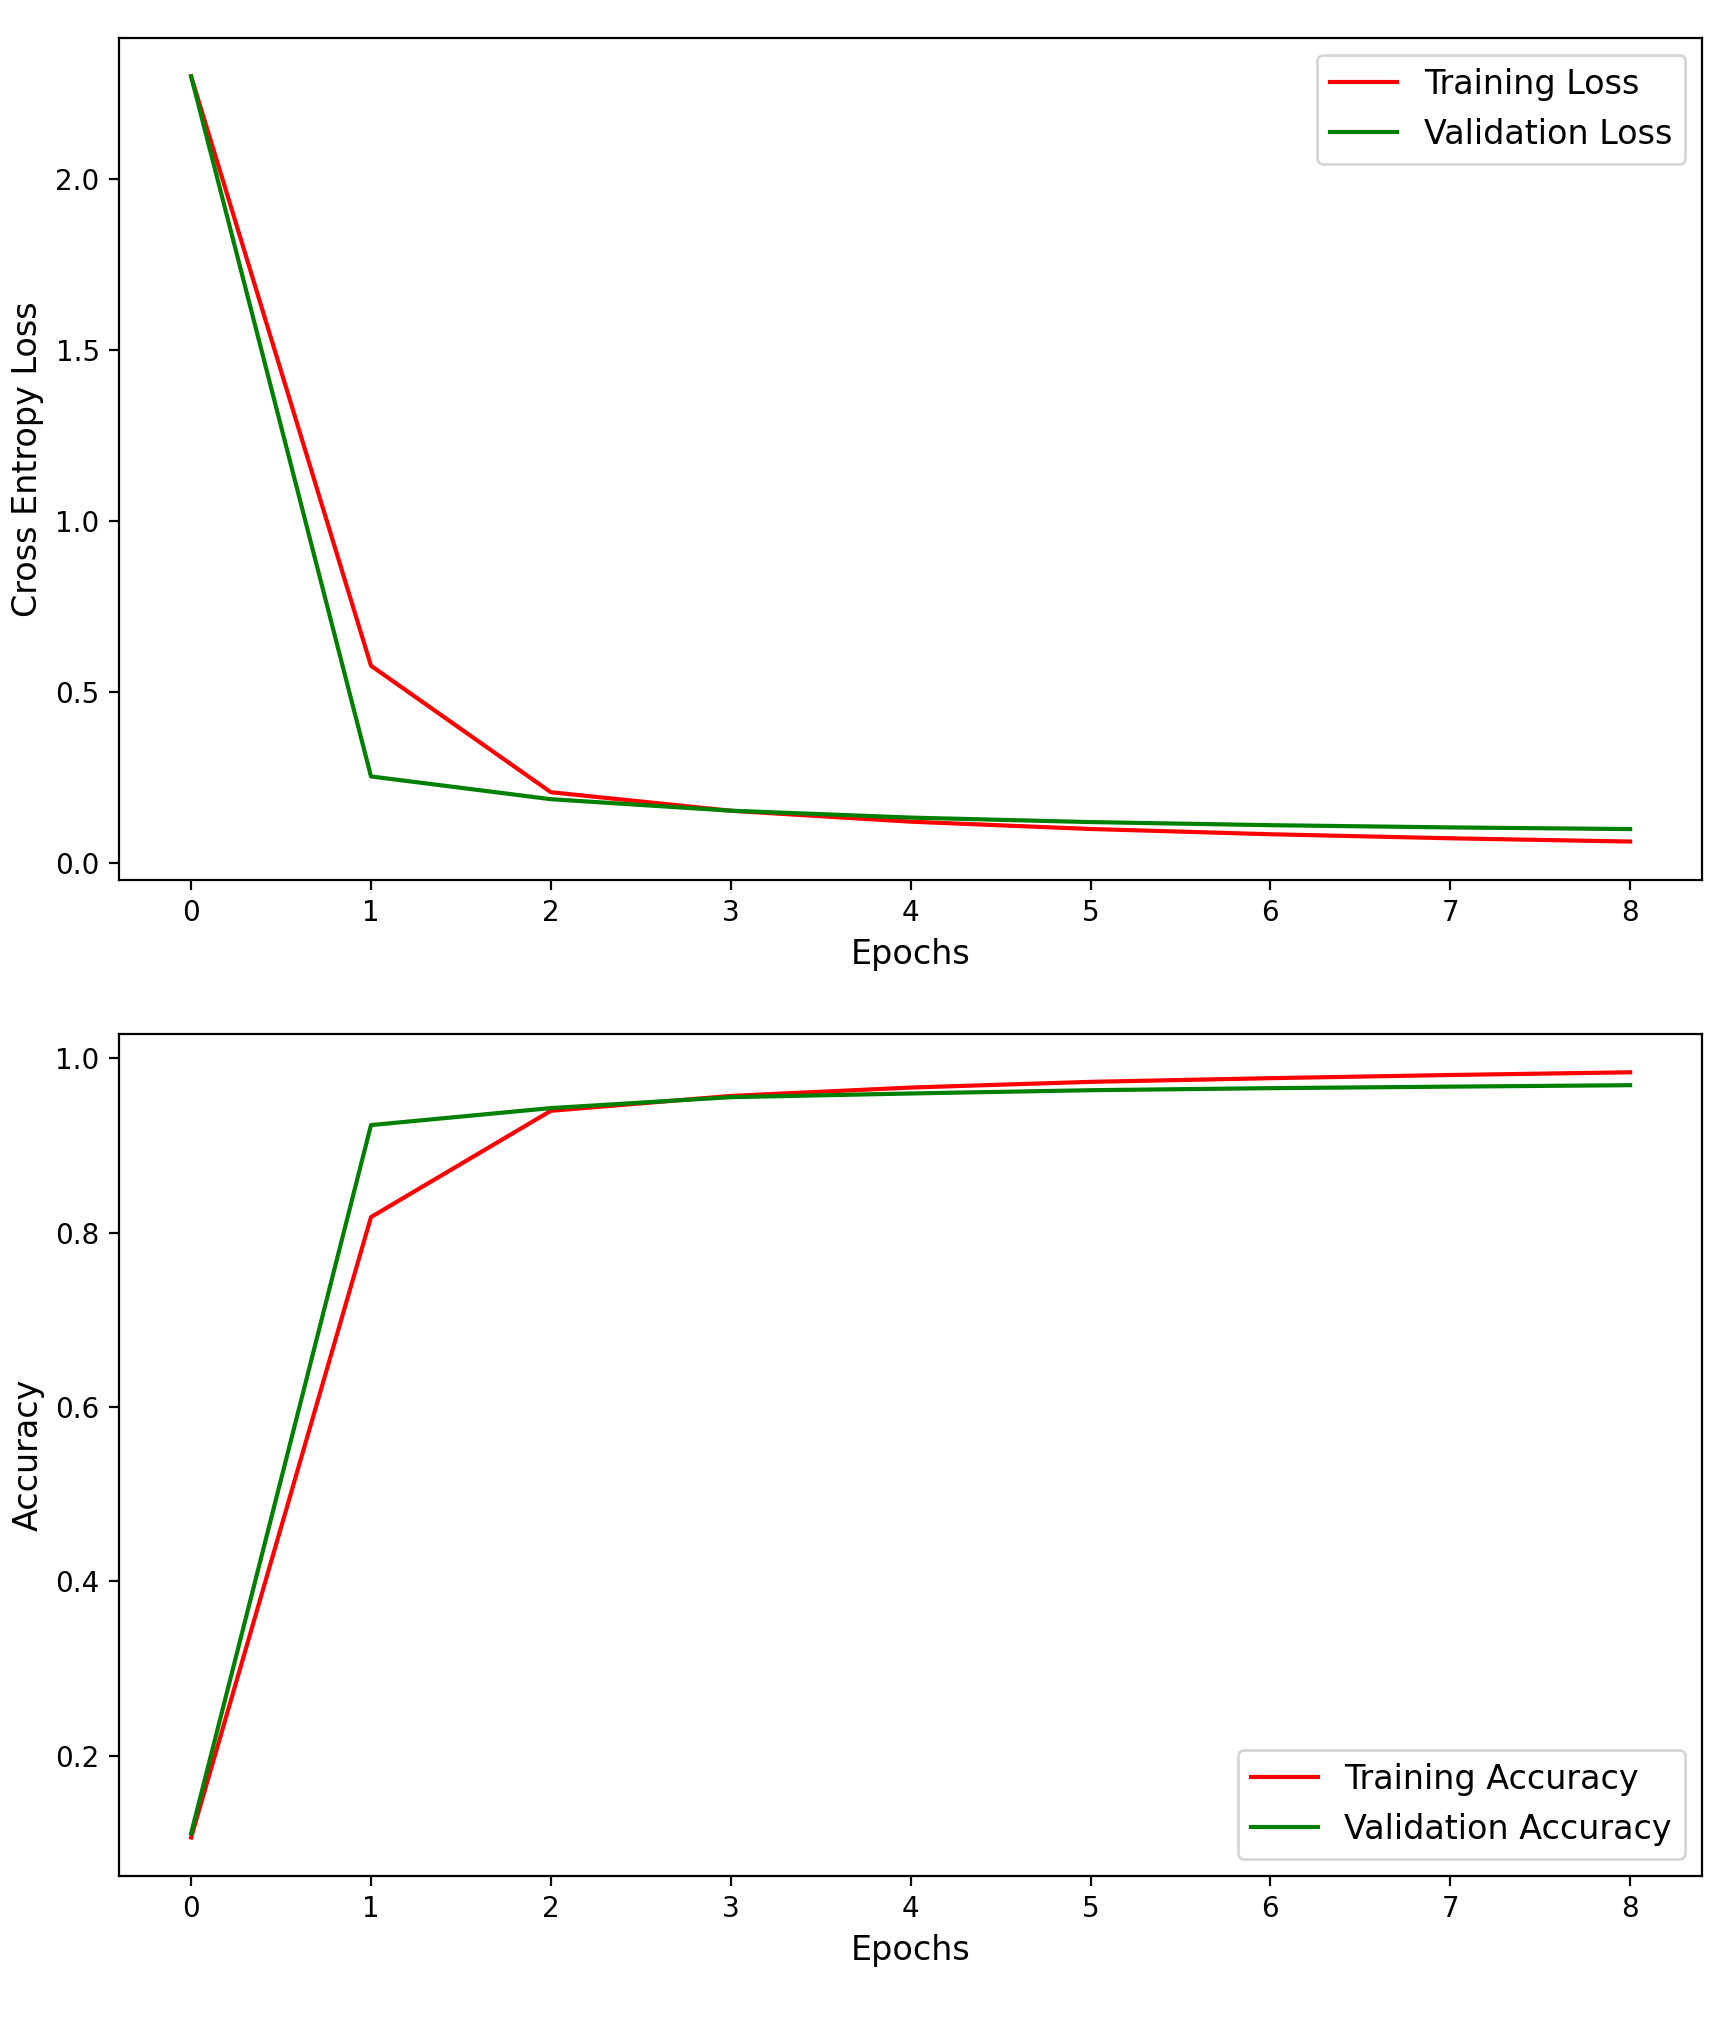
\includegraphics[width=1.0\textwidth]{./images/l1_e4.png}
	\caption{$L_1$ Regularization with $\lambda = 1e^{-4}$}
	\label{fig:l1_1e4}
\end{figure}

\begin{figure}[!ht]
	\centering
	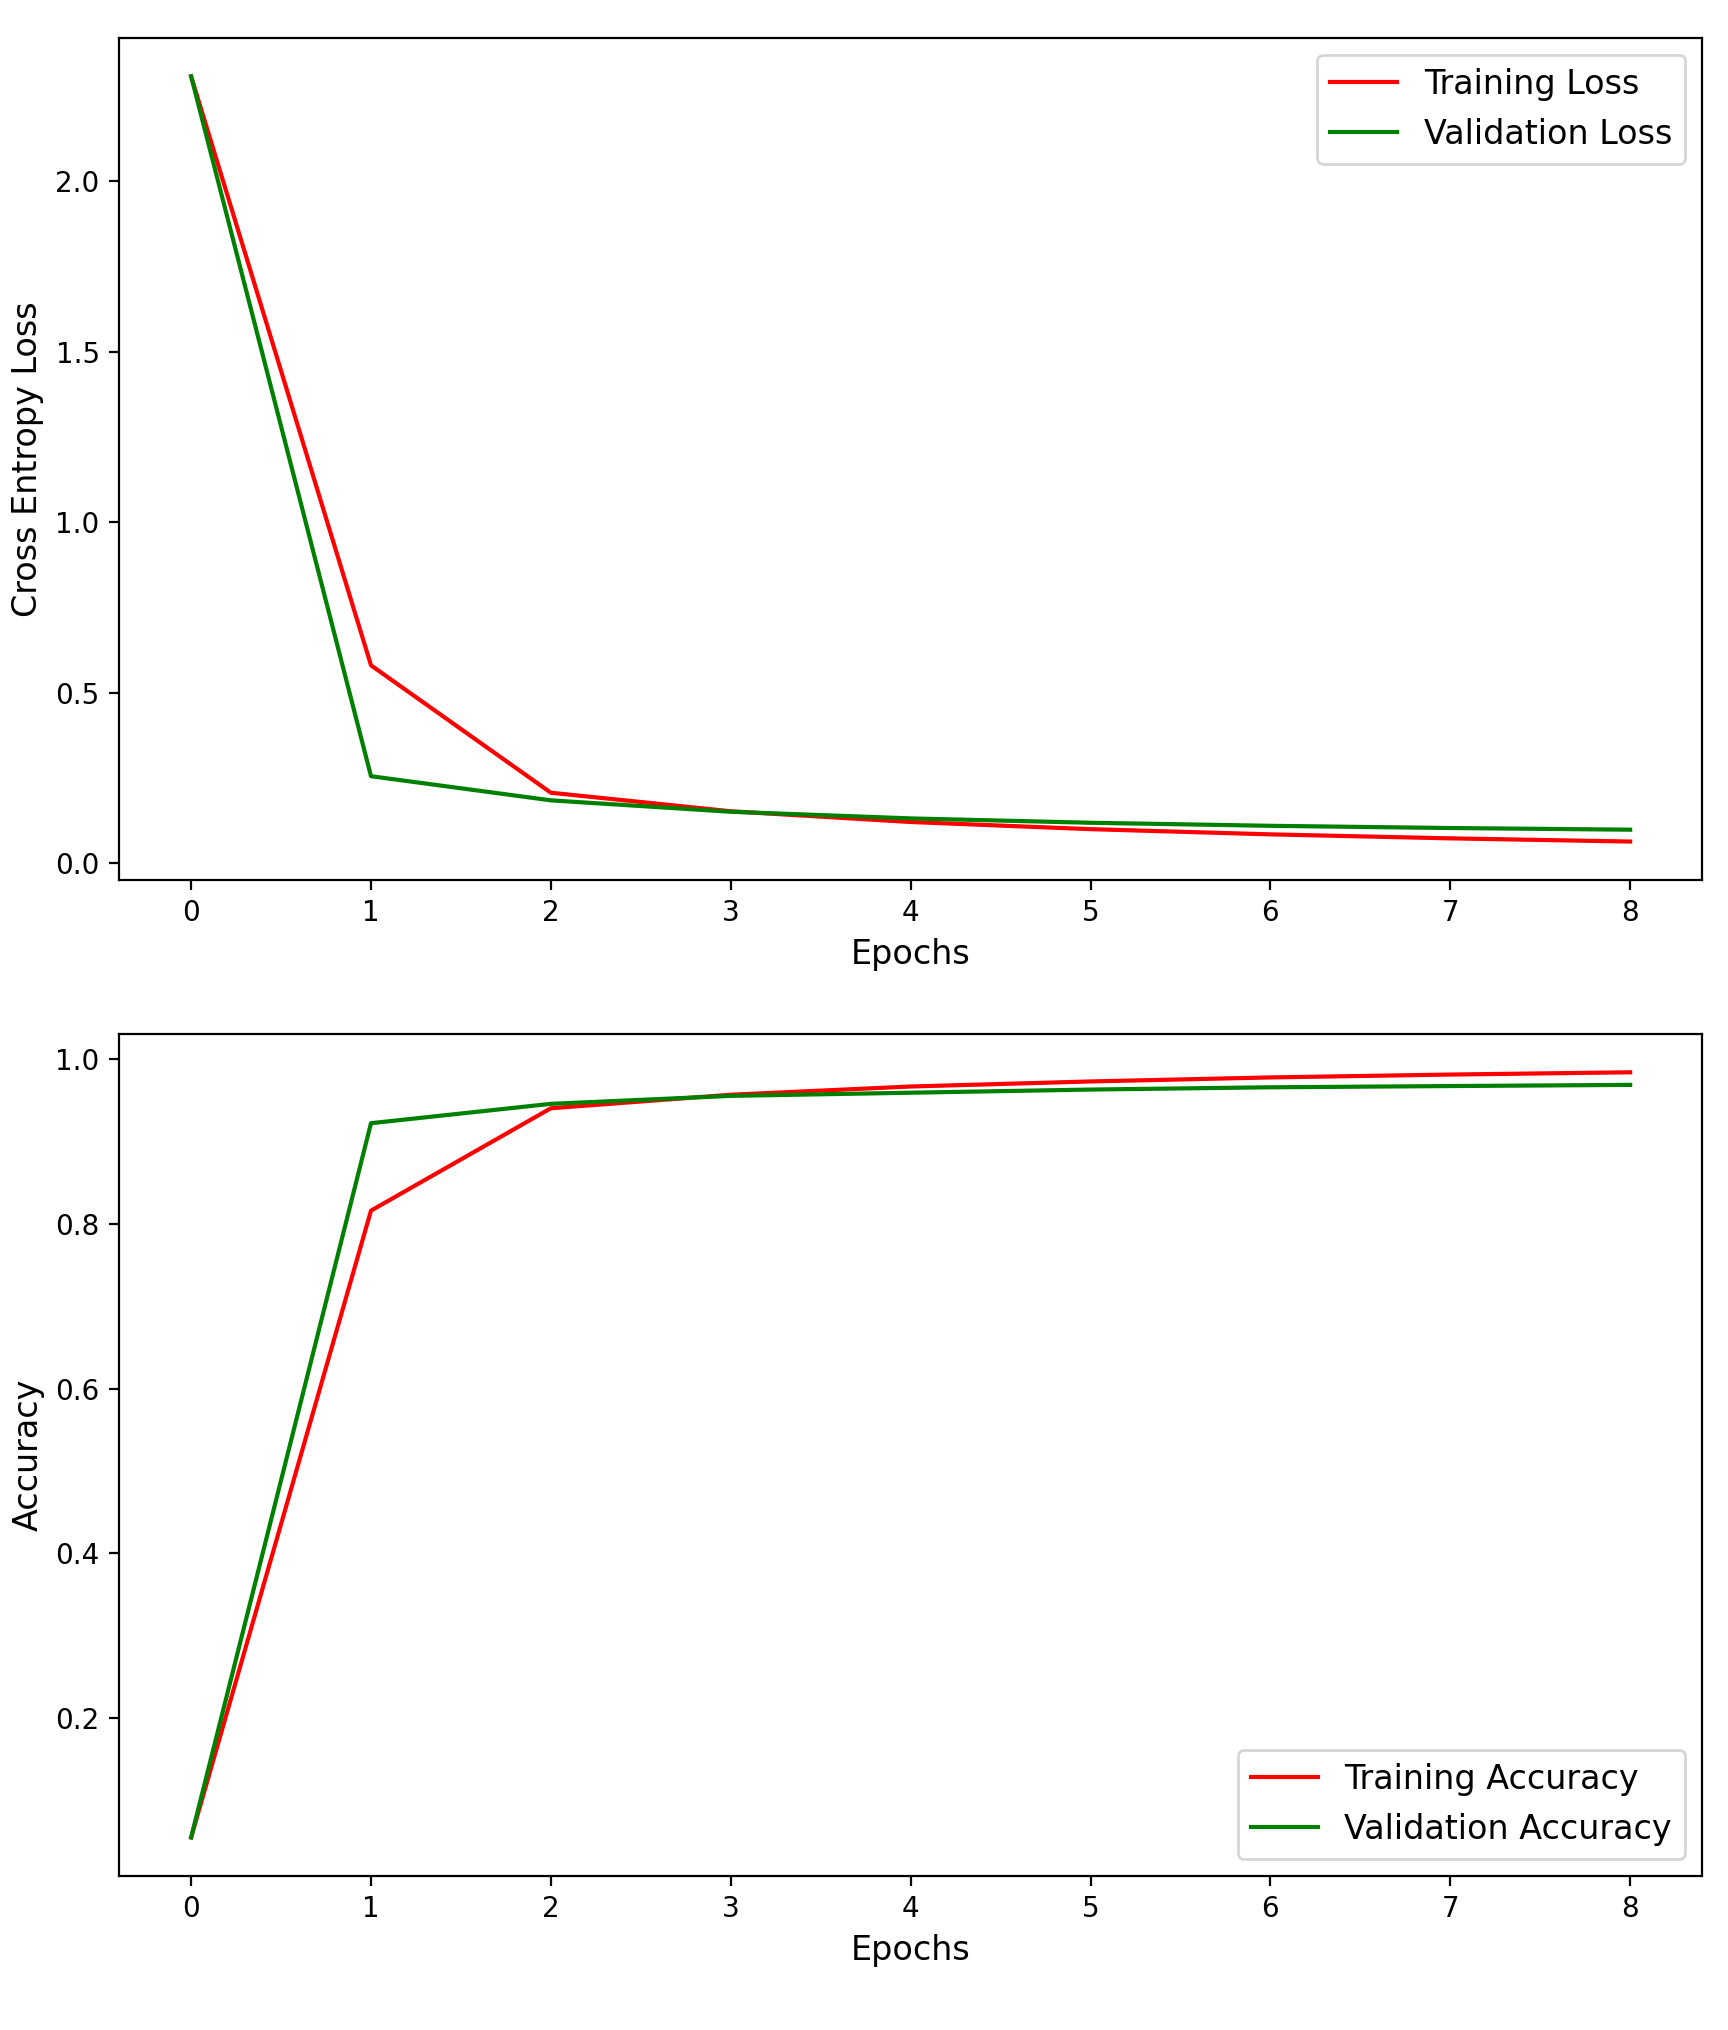
\includegraphics[width=1.0\textwidth]{./images/l2_e2.png}
	\caption{$L_2$ Regularization with $\lambda = 1e^{-2}$}
	\label{fig:l2_1e2}
\end{figure}

\begin{figure}[!ht]
	\centering
	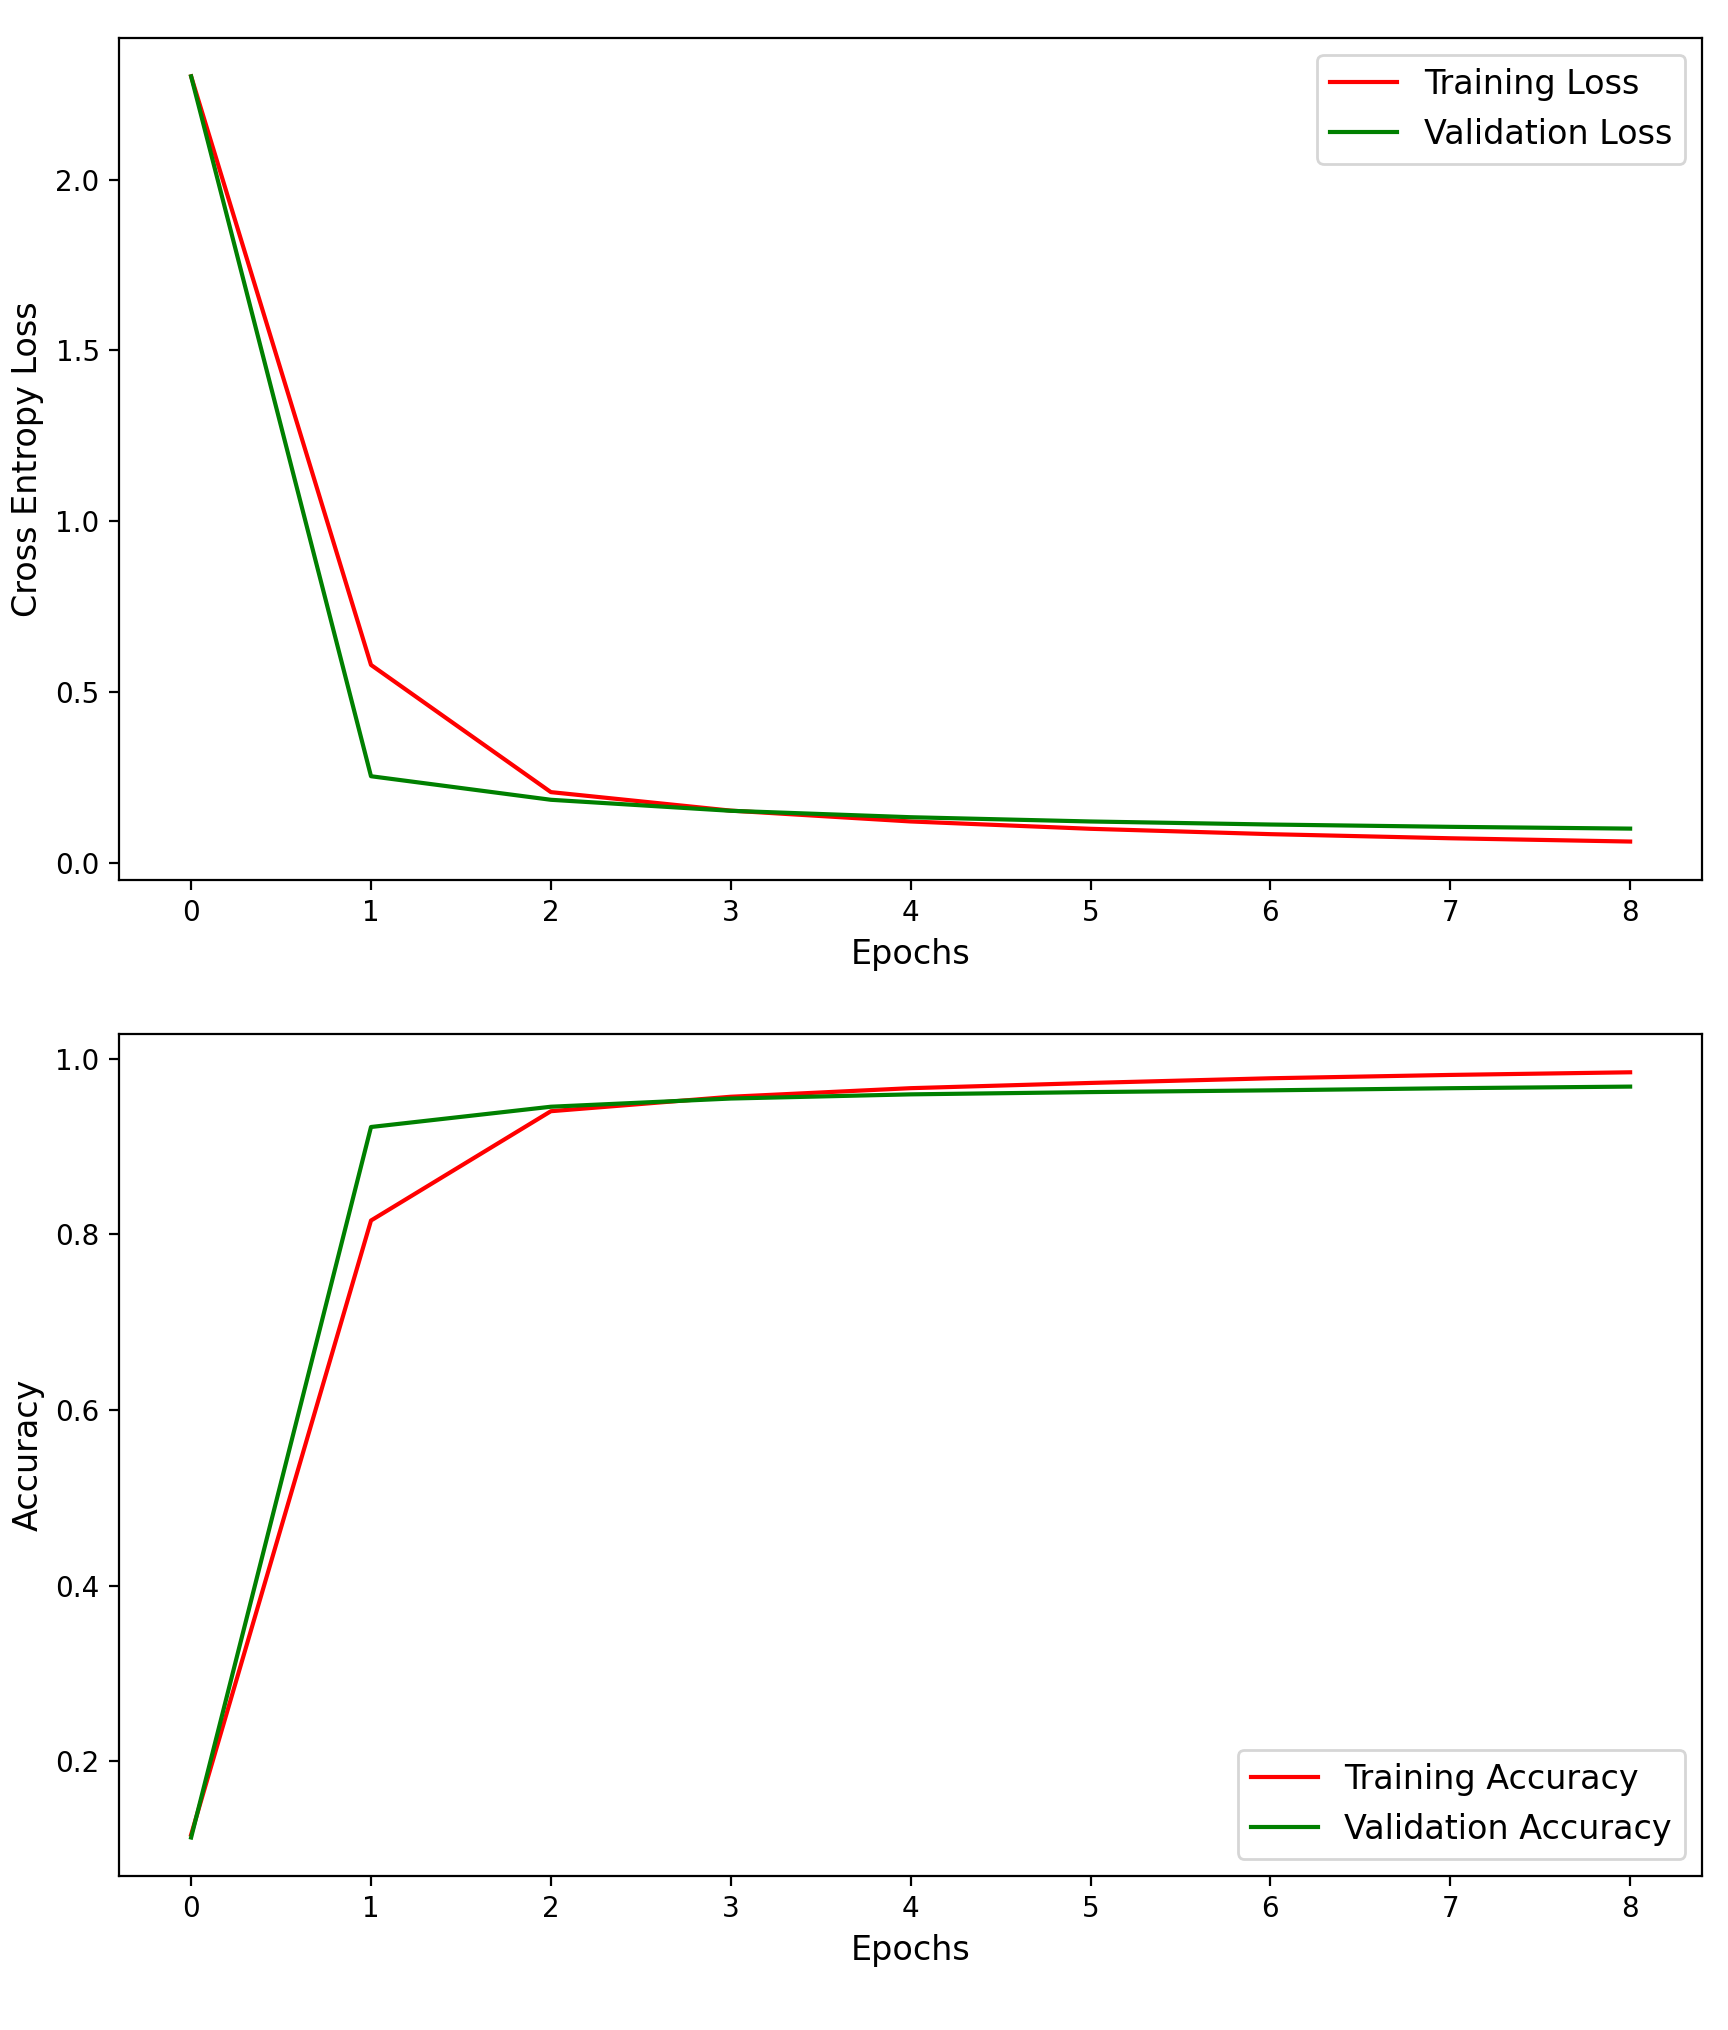
\includegraphics[width=1.0\textwidth]{./images/l2_e4.png}
	\caption{$L_2$ Regularization with $\lambda = 1e^{-4}$}
	\label{fig:l2_1e4}
\end{figure}
